% !TEX encoding = UTF-8 Unicode
% !TEX TS-program = xelatex

\chapter{排列組合相關圖形}
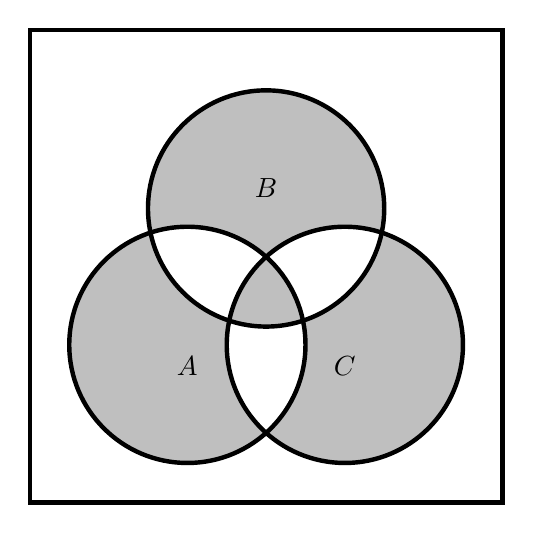
\begin{tikzpicture}
\def\firstcircle{(0,0) circle (1.5cm)}
\def\secondcircle{(60:2cm) circle (1.5cm)}
\def\thirdcircle{(0:2cm) circle (1.5cm)}

% Now we want to highlight the intersection of the first and the
% second circle:
\begin{scope}
\fill [lightgray] \firstcircle;
\end{scope}
\begin{scope}
\fill [lightgray] \secondcircle;
\end{scope}
\begin{scope}
\fill [lightgray] \thirdcircle;
\end{scope}


\begin{scope}
\clip \firstcircle;
\fill[white] \secondcircle;
\end{scope}
\begin{scope}
\clip \secondcircle;
\fill[white] \thirdcircle;
\end{scope}

\begin{scope}
\clip \thirdcircle;
\fill[white] \firstcircle;
\end{scope}

% Next, we want the highlight the intersection of all three circles:

\begin{scope}
\clip \firstcircle;
\clip \secondcircle;
\fill[lightgray] \thirdcircle;
\end{scope}

\draw [ultra thick] \firstcircle node[below] {$A$};
\draw [ultra thick] \secondcircle node [above] {$B$};
\draw [ultra thick] \thirdcircle node [below] {$C$};

\draw [ultra thick] (-2cm,-2cm) rectangle  (4cm,4cm);

\end{tikzpicture}

    \begin{tikzpicture}

\foreach \v in {0,1}
{
    \foreach \u in {0,1,2}
    {
        \draw[ultra thick] (\v,\u) -- (\v,{\u+1}) -- ({\v+1},{\u+1}) -- ({\v+1},{\u}) -- (\v,\u) circle;
    };
};
\coordinate (cAPt) at (0,0);
\coordinate (cBPt) at (2,3);
\coordinate (cCPt) at (1,2);
\coordinate (cDPt) at (1,3);
\coordinate (cEPt) at (2,2);

\foreach \v/\u/\t in 
{cAPt/180/$A$,
    cBPt/90/$B$,
    cDPt/90/$D$,
    cCPt/225/$C$,
    cEPt/0/$E$}
{
    \draw[ultra thick,fill] (\v) circle (2pt);
    \node[label=\u:\t] at (\v){};
    
};
\begin{scope}[shift={(3,2)}]
\draw[ultra thick,-latex] (0,0) -- (0,1) ;
\draw[ultra thick,-latex] (0,0) -- (1,0) ;
\node [label=0:東] at (1,0){};
\node [label=90:北] at (0,1){};

\end{scope}
\end{tikzpicture}

    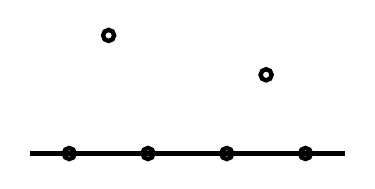
\begin{tikzpicture}

\draw [ultra thick](0.5,0) -- (4.5,0);

\draw[ultra thick] (1,0) circle (2pt);
\draw[ultra thick] (2,0) circle (2pt);
\draw[ultra thick] (3,0) circle (2pt);
\draw[ultra thick] (4,0) circle (2pt);
\draw[ultra thick] (1.5,1.5) circle (2pt);
\draw[ultra thick] (3.5,1) circle (2pt);
\end{tikzpicture}

\begin{tikzpicture}[scale=1]
\newcommand{\HOfLine}{0.3};
\foreach \v in 
{0,...,3}
{
    \draw  ({-0.5  } , {0.5+\HOfLine*\v})  -- ({6}, {0.5+\HOfLine*\v});
}

\foreach \v in 
{0,...,3}
{
    \draw  ({0 +  \HOfLine*\v} , {0})  -- ({3.5+\HOfLine*\v}, {5});
}

\foreach \v in 
{0,...,3}
{
    \draw  ({4.5 +  \HOfLine*\v} , {0})  -- ({1.5+\HOfLine*\v}, {5});
}
\end{tikzpicture}

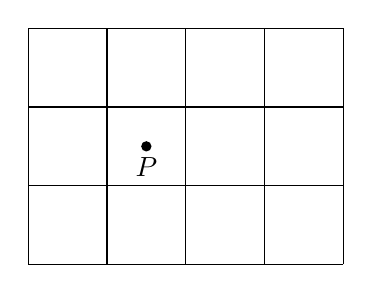
\begin{tikzpicture}[scale=1]

\coordinate (cPPt) at (1.5,1.5);
\draw[color=black] (0,0) grid (4,3);
\draw[ultra thick,fill] (cPPt) circle (1pt) node[ below ]  {$P$};

\end{tikzpicture}


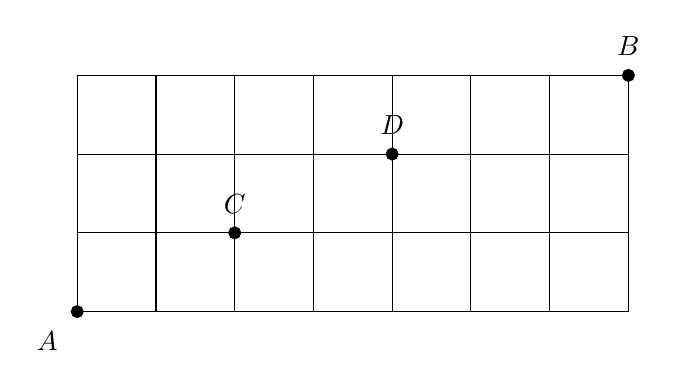
\begin{tikzpicture}[scale=1]

\coordinate (cAPt) at (0,0);
\coordinate (cBPt) at (7,3);
\coordinate (cCPt) at (2,1);
\coordinate (cDPt) at (4,2);
\draw[color=black] (0,0) grid (7,3);
%\draw[ultra thick,fill] (cPPt) circle (1pt) node[ below ]  {$P$};
\foreach \v/\u/\t in 
{   cAPt/225/$A$,
    cBPt/90 /$B$,
    cCPt/90 /$C$,
    cDPt/90 /$D$
}
{
    \draw[ultra thick,fill] (\v) circle (1.5pt);
    \node[label=\u:\t] at (\v){};
}; 

\end{tikzpicture}

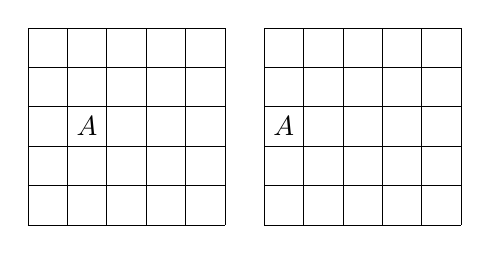
\begin{tikzpicture}[scale=.5]
\draw[very thin,color=black] (0,0) grid (5,5);

\def\seatSymbol{$\CIRCLE$}

\node at (1.5,2.5 ) {$A$};
\node at (1.5,3.5 ) {\seatSymbol};
\node at (1.5, 1.5) {\seatSymbol};
\node at (0.5,2.5) {\seatSymbol};
\node at (2.5, 2.5) {\seatSymbol};

\begin{scope}[shift={(6,0)}]
\draw[very thin,color=black] (0,0) grid (5,5);
\node at (0.5,2.5 ) {$A$};
\node at (0.5,3.5 ) {\seatSymbol};
\node at (0.5, 1.5) {\seatSymbol};
\node at (1.5, 2.5) {\seatSymbol};
\end{scope}
\end{tikzpicture}
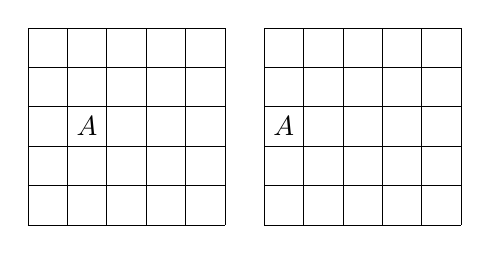
\begin{tikzpicture}[scale=.5]
\draw[very thin,color=black] (0,0) grid (5,5);

\def\seatSymbol{$\CIRCLE$}

\node at (1.5,2.5 ) {$A$};
\node at (1.5,3.5 ) {\seatSymbol};
\node at (1.5, 1.5) {\seatSymbol};
\node at (0.5,2.5) {\seatSymbol};
\node at (2.5, 2.5) {\seatSymbol};

\begin{scope}[shift={(6,0)}]
\draw[very thin,color=black] (0,0) grid (5,5);
\node at (0.5,2.5 ) {$A$};
\node at (0.5,3.5 ) {\seatSymbol};
\node at (0.5, 1.5) {\seatSymbol};
\node at (1.5, 2.5) {\seatSymbol};
\end{scope}
\end{tikzpicture}

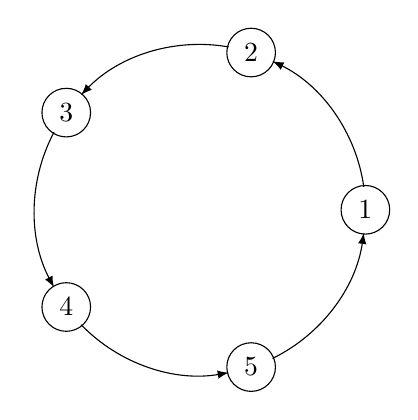
\begin{tikzpicture}[scale=0.7]

\def \n {5}
\def \radius {3cm}
\def \margin {8} % margin in angles, depends on the radius

\foreach \s in {1,...,\n}
{
    \node[draw, circle] at ({360/\n * (\s - 1)}:\radius) {$\s$};
    \draw[->, >=latex] ({360/\n * (\s - 1)+\margin}:\radius) 
    arc ({360/\n * (\s - 1)+\margin}:{360/\n * (\s)-\margin}:\radius);
}
\end{tikzpicture}


    \begin{tikzpicture}

\begin{scope}[shift={(0,0)}]
{
    \filldraw[fill=lightgray,draw=black] (0,0) rectangle (2,1);
    \draw[dashed] (1,0) -- (1,1);
    \node[above] at (0.5,1){積木};
}
\end{scope}
\begin{scope}[shift={(4,0)}]
\node[above] at (0.5,1){底板};
\foreach \x in {0,...,11}
{
    \begin{scope}[shift={(\x, 0)}]
    \filldraw[fill=white,draw=black] (0,0) rectangle (1,1);
    \end{scope}
}
\end{scope}

\end{tikzpicture}